\documentclass[10pt,letterpaper]{article}
\usepackage[margin=0.65in,headheight=14pt,footskip=22pt]{geometry}
\usepackage[T1]{fontenc}
\usepackage{lmodern,microtype}
\usepackage{xcolor,tikz,enumitem,fancyhdr,hyperref}
\usetikzlibrary{arrows.meta,positioning,calc}
\hypersetup{colorlinks=true,urlcolor=blue!55!black,linkcolor=blue!55!black,
pdftitle={ReturnFlow: Midpoint Architecture},pdfauthor={Zejun Xu, Peixuan Ji, Shuchen Liu}}
\newcommand{\TeamMembers}{Zejun Xu, Peixuan Ji, Shuchen Liu}
\newcommand{\ReportDate}{October 25, 2026}
\newcommand{\RepoURL}{https://github.com/Zejun-Derry-Xu/DML_Project}
% Midpoint report source, kept at the repository root for easy access.
% Public entry verified for the deployed course demo on October 25, 2026.
\newcommand{\ApplicationURL}{https://http-149-165-169-223-5173.proxy-js2-iu.exosphere.app/}
\definecolor{ink}{HTML}{19384A}
\definecolor{live}{HTML}{285FB6}
\definecolor{semantic}{HTML}{7046A0}
\definecolor{rule}{HTML}{A15B10}
\definecolor{storage}{HTML}{237865}
\definecolor{bluewash}{HTML}{EDF3FB}
\definecolor{goldwash}{HTML}{FCF3E6}
\definecolor{greenwash}{HTML}{EDF5F0}
\definecolor{muted}{HTML}{53616D}
\definecolor{purplewash}{HTML}{F3EDF9}
\definecolor{redwash}{HTML}{FBEFF0}
\definecolor{statewash}{HTML}{F2F4F7}
\color{ink}
\setlength{\parindent}{0pt}\setlength{\parskip}{5pt}
\setlist[itemize]{leftmargin=1.2em,itemsep=2pt,topsep=3pt}
\pagestyle{fancy}\fancyhf{}
\fancyhead[L]{\small\textbf{ReturnFlow} / DSAN 6700}
\fancyhead[R]{\small Midpoint architecture / Deployed prototype}
\fancyfoot[L]{\footnotesize\ReportDate}
\fancyfoot[R]{\footnotesize\thepage\ / \pageref*{report-end}}
\renewcommand{\headrulewidth}{0.3pt}
\newcommand{\heading}[1]{\vspace{3pt}{\large\bfseries #1}\par\vspace{2pt}}
\newcommand{\notice}[1]{\begingroup\setlength{\fboxsep}{7pt}
\colorbox{goldwash}{\parbox{\dimexpr\linewidth-14pt\relax}{\small #1}}\endgroup\par}
\newcommand{\code}[1]{\texttt{\small\detokenize{#1}}}
\newcommand{\semanticspan}[1]{\textcolor{semantic}{\textbf{#1}}}
\newcommand{\action}[1]{\textcolor{live}{\textbf{#1}}}
\newcommand{\fixedrule}[1]{\textcolor{rule}{\textbf{#1}}}
\newcommand{\examplequote}[1]{\begingroup\setlength{\fboxsep}{8pt}
\colorbox{bluewash}{\parbox{\dimexpr\linewidth-16pt\relax}{\large\raggedright
\textquotedblleft{}#1\textquotedblright{}}}\endgroup\par}
\tikzset{
box/.style={draw=ink!40,rounded corners=4pt,fill=white,align=center,
font=\sffamily\small,inner sep=6pt,minimum height=1.0cm},
smallbox/.style={box,font=\sffamily\footnotesize,inner sep=5pt},
request/.style={-{Stealth[length=2mm]},draw=live,line width=1pt},
modelpath/.style={-{Stealth[length=2mm]},draw=semantic,line width=1pt},
label/.style={font=\sffamily\footnotesize,text=muted,align=center},
layer/.style={rounded corners=3pt,draw=ink!22,line width=.5pt},
layername/.style={anchor=west,font=\sffamily\bfseries\footnotesize},
module/.style={box,font=\sffamily\footnotesize,inner sep=5pt,minimum height=.95cm},
opsflow/.style={-{Stealth[length=1.7mm]},draw=rule!85,dashed,line width=.7pt},
releaseflow/.style={-{Stealth[length=1.7mm]},draw=storage,dashed,line width=.7pt},
edgehint/.style={font=\sffamily\scriptsize,fill=white,inner sep=2pt,align=center,text=ink}}

\begin{document}
{\LARGE\bfseries ReturnFlow: describe the return, not the form}\par
\textbf{Team:} \TeamMembers\hfill\textbf{Midpoint check-in}\par
\textbf{Repository:} \url{\RepoURL}\par
\textbf{Jetstream2 course demo (public entry verified October 25):}\par
{\small\url{\ApplicationURL}}\par
\notice{Our checklist-led prototype is deployed on Jetstream2 with Qwen3 4B.
This midpoint report focuses on the user journey, service architecture and repeatable
delivery process. All accounts, support tickets and return requests are simulated;
no real payments or refunds are processed.}

\heading{1. Solution architecture: a conversation with a clear finish}
A customer should be able to say what went wrong in their own words instead of
learning the store's internal return form. ReturnFlow turns that description into
candidate facts, checks the customer's order, and explains the conditions that matter.
Because customers cannot be expected to volunteer every policy detail, the interface
shows the remaining conditions together. They can answer them collectively or describe
an exception; they do not need to complete a separate card for every condition.

\begin{center}
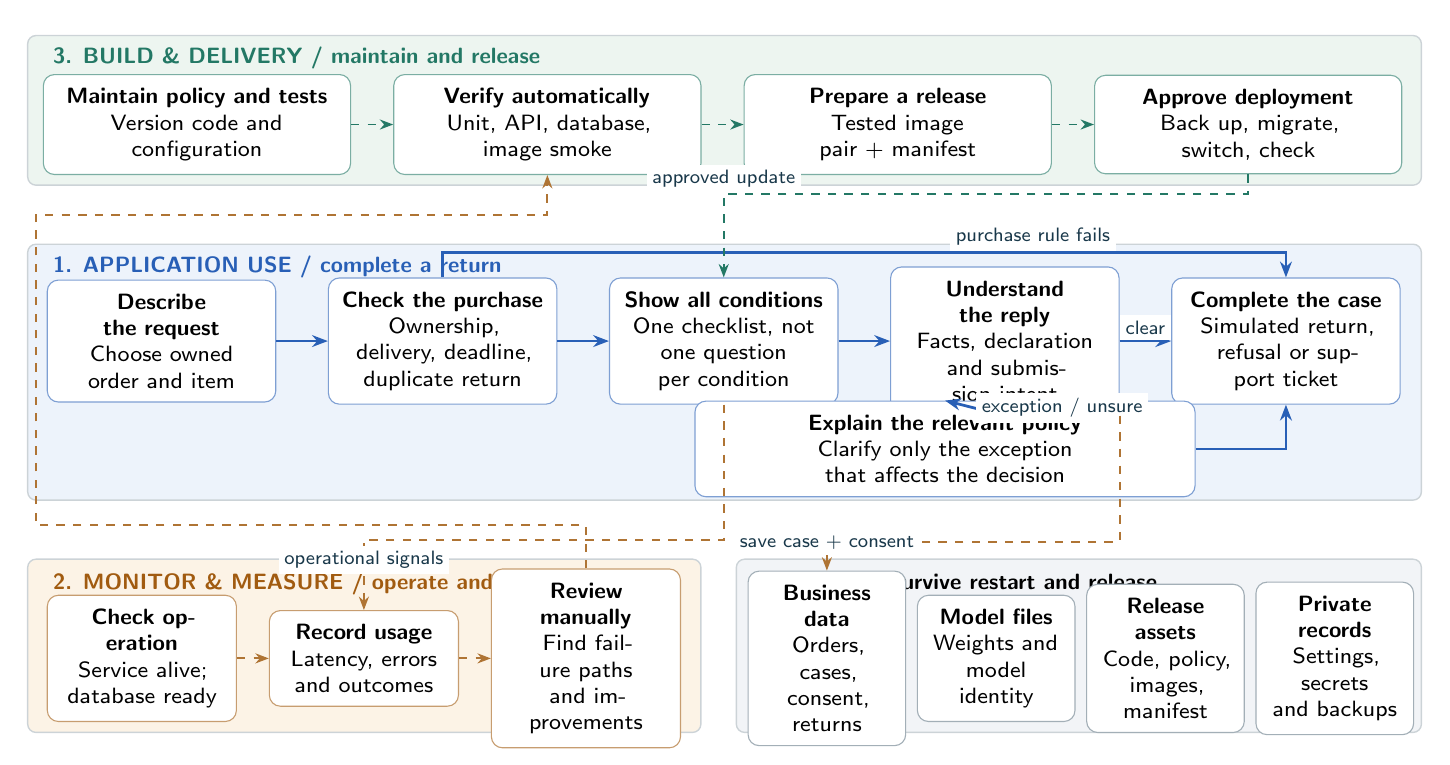
\begin{tikzpicture}[x=1cm,y=1cm]
\path[use as bounding box] (0,-8.9) rectangle (17.7,.1);
\draw[layer,fill=greenwash] (0,0) rectangle (17.7,-1.9);
\node[layername,text=storage] at (.2,-.28) {3. BUILD \& DELIVERY / maintain and release};
\node[module,text width=3.55cm,draw=storage!60] (maintain) at (2.15,-1.13)
{\textbf{Maintain policy and tests}\\Version code and configuration};
\node[module,text width=3.55cm,draw=storage!60] (verify) at (6.6,-1.13)
{\textbf{Verify automatically}\\Unit, API, database, image smoke};
\node[module,text width=3.55cm,draw=storage!60] (package) at (11.05,-1.13)
{\textbf{Prepare a release}\\Tested image pair + manifest};
\node[module,text width=3.55cm,draw=storage!60] (deploy) at (15.5,-1.13)
{\textbf{Approve deployment}\\Back up, migrate, switch, check};
\draw[releaseflow] (maintain)--(verify);
\draw[releaseflow] (verify)--(package);
\draw[releaseflow] (package)--(deploy);

\draw[layer,fill=bluewash] (0,-2.65) rectangle (17.7,-5.9);
\node[layername,text=live] at (.2,-2.94) {1. APPLICATION USE / complete a return};
\node[module,text width=2.55cm,draw=live!60] (describe) at (1.7,-3.88)
{\textbf{Describe the request}\\Choose owned order and item};
\node[module,text width=2.55cm,draw=live!60] (purchase) at (5.27,-3.88)
{\textbf{Check the purchase}\\Ownership, delivery, deadline,\\duplicate return};
\node[module,text width=2.55cm,draw=live!60] (conditions) at (8.84,-3.88)
{\textbf{Show all conditions}\\One checklist, not\\one question per condition};
\node[module,text width=2.55cm,draw=live!60] (understand) at (12.41,-3.88)
{\textbf{Understand the reply}\\Facts, declaration\\and submission intent};
\node[module,text width=2.55cm,draw=live!60] (finish) at (15.98,-3.88)
{\textbf{Complete the case}\\Simulated return,\\refusal or support ticket};
\draw[request] (describe)--(purchase);
\draw[request] (purchase)--(conditions);
\draw[request] (conditions)--(understand);
\draw[request] (understand)--node[edgehint,above] {clear}(finish);
\node[module,text width=6.0cm,minimum height=.85cm,draw=live!60] (explain) at (11.65,-5.25)
{\textbf{Explain the relevant policy}\\Clarify only the exception that affects the decision};
\draw[request] (understand.south)--node[edgehint,right] {exception / unsure}(explain.north);
\draw[request] (explain.east)-|(finish.south);
\draw[request] (purchase.north)--++(0,.32)-|node[edgehint,pos=.35,above]
{purchase rule fails}(finish.north);
\draw[releaseflow] (deploy.south)--++(0,-.25)-|node[edgehint,pos=.5,above]
{approved update}(conditions.north);

\draw[layer,fill=goldwash] (0,-6.65) rectangle (8.55,-8.85);
\node[layername,text=rule] at (.2,-6.96) {2. MONITOR \& MEASURE / operate and improve};
\node[module,text width=2.05cm,draw=rule!60] (health) at (1.45,-7.91)
{\textbf{Check operation}\\Service alive;\\database ready};
\node[module,text width=2.05cm,draw=rule!60] (usage) at (4.27,-7.91)
{\textbf{Record usage}\\Latency, errors\\and outcomes};
\node[module,text width=2.05cm,draw=rule!60] (review) at (7.09,-7.91)
{\textbf{Review manually}\\Find failure paths\\and improvements};
\draw[opsflow] (health)--(usage);
\draw[opsflow] (usage)--(review);
\draw[opsflow] (conditions.south)--++(0,-1.72)-|node[edgehint,pos=.75,above]
{operational signals}(usage.north);
\draw[opsflow] (review.north)--++(0,.55)-|(.1,-2.28)-|(verify.south);

\draw[layer,fill=statewash] (9,-6.65) rectangle (17.7,-8.85);
\node[layername] at (9.2,-6.96) {4. STATE / survive restart and release};
\node[module,text width=1.65cm] (business) at (10.15,-7.91)
{\textbf{Business data}\\Orders, cases,\\consent, returns};
\node[module,text width=1.65cm] at (12.3,-7.91)
{\textbf{Model files}\\Weights and\\model identity};
\node[module,text width=1.65cm] (assets) at (14.45,-7.91)
{\textbf{Release assets}\\Code, policy,\\images, manifest};
\node[module,text width=1.65cm] at (16.6,-7.91)
{\textbf{Private records}\\Settings, secrets\\and backups};
\draw[opsflow] (understand.south east)--++(0,-1.6)-|node[edgehint,pos=.75,above]
{save case + consent}(business.north);
\end{tikzpicture}
\end{center}
{\footnotesize Blue solid: customer request path.\quad
Green dashed: release flow.\quad Amber dashed: records and operational feedback.}

The intended normal path has a clear finish: after the order checks and checklist,
\emph{none of these problems apply, and submit} expresses the declaration and submission
request together. Saying only \emph{all clear} does not authorize submission. If tags
were removed or a condition is uncertain, the system explains the relevant policy and
asks only what is needed to resolve that exception. It never promises a real refund.

The same design covers the application's lifecycle. Developers maintain a versioned
policy and test the application before promoting a release. During use, the frontend
displays the conversation, owned-order choices and current checklist while the backend
controls the next step. After use, request logs, health checks and latency metrics help
the team find operational problems. PostgreSQL keeps the case, answers, checklist
snapshot, consent, simulated returns and tickets across refreshes. Model weights live
in a separate volume; code, policy and image versions are tracked in Git and the
registry, while secrets and backups remain private.

\newpage
\heading{2. Technical architecture: four services, separate responsibilities}
We use one CPU-only Jetstream2 VM and Docker Compose rather than several agent
services. The web server displays the interface, the application server runs the
return workflow, PostgreSQL saves its state, and Ollama serves Qwen3 4B to interpret
language. A policy file and clause search run \emph{inside} the application server;
they are not additional containers.

\begin{center}
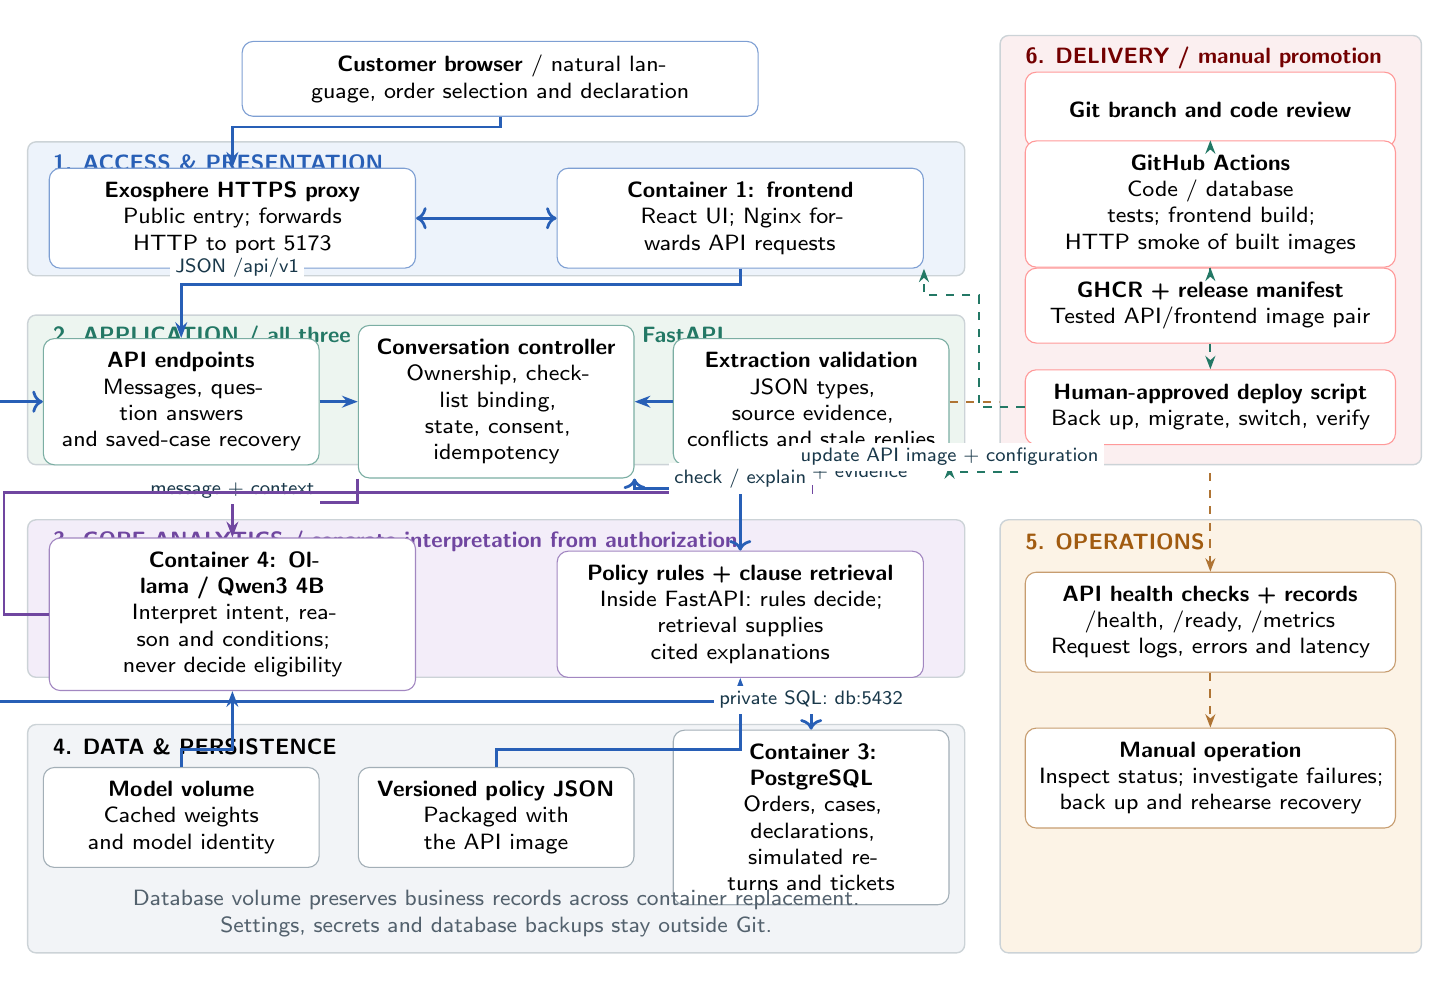
\begin{tikzpicture}[x=1cm,y=1cm]
\path[use as bounding box] (0,-11.7) rectangle (17.7,.1);
\node[module,text width=6.2cm,draw=live!60] (browser) at (6.0,-.55)
{\textbf{Customer browser} / natural language, order selection and declaration};
\draw[layer,fill=bluewash] (0,-1.35) rectangle (11.9,-3.05);
\node[layername,text=live] at (.2,-1.62) {1. ACCESS \& PRESENTATION};
\node[module,text width=4.3cm,draw=live!60] (proxy) at (2.6,-2.32)
{\textbf{Exosphere HTTPS proxy}\\Public entry; forwards HTTP to port 5173};
\node[module,text width=4.3cm,draw=live!60] (web) at (9.05,-2.32)
{\textbf{Container 1: frontend}\\React UI; Nginx forwards API requests};
\draw[request] (browser.south)--++(0,-.13)-|(proxy.north);
\draw[request,<->] (proxy)--(web);

\draw[layer,fill=greenwash] (0,-3.55) rectangle (11.9,-5.45);
\node[layername,text=storage] at (.2,-3.83) {2. APPLICATION / all three modules share container 2: FastAPI};
\node[module,text width=3.15cm,draw=storage!60] (api) at (1.95,-4.65)
{\textbf{API endpoints}\\Messages, question answers\\and saved-case recovery};
\node[module,text width=3.15cm,draw=storage!60] (workflow) at (5.95,-4.65)
{\textbf{Conversation controller}\\Ownership, checklist binding,\\state, consent, idempotency};
\node[module,text width=3.15cm,draw=storage!60] (validate) at (9.95,-4.65)
{\textbf{Extraction validation}\\JSON types, source evidence,\\conflicts and stale replies};
\draw[request] (web.south)--++(0,-.2)-|node[edgehint,pos=.45,above]
{JSON /api/v1}(api.north);
\draw[request] (api)--(workflow);
\draw[request] (validate)--(workflow);

\draw[layer,fill=purplewash] (0,-6.15) rectangle (11.9,-8.15);
\node[layername,text=semantic] at (.2,-6.43) {3. CORE ANALYTICS / separate interpretation from authorization};
\node[module,text width=4.3cm,draw=semantic!65] (model) at (2.6,-7.35)
{\textbf{Container 4: Ollama / Qwen3 4B}\\Interpret intent, reason and conditions;\\never decide eligibility};
\node[module,text width=4.3cm,draw=semantic!65] (policy) at (9.05,-7.35)
{\textbf{Policy rules + clause retrieval}\\Inside FastAPI: rules decide;\\retrieval supplies cited explanations};
\draw[modelpath] (workflow.south west)--++(0,-.3)-|node[edgehint,pos=.55,above]
{message + context}(model.north);
\draw[modelpath] (model.west)--(-.3,-7.35)--(-.3,-5.8)-|node[edgehint,pos=.6,above]
{candidates + evidence}(validate.south);
\draw[request,<->] (workflow.south east)--++(0,-.13)-|node[edgehint,pos=.55,above]
{check / explain}(policy.north);

\draw[layer,fill=statewash] (0,-8.75) rectangle (11.9,-11.65);
\node[layername] at (.2,-9.03) {4. DATA \& PERSISTENCE};
\node[module,text width=3.15cm] (weights) at (1.95,-9.93)
{\textbf{Model volume}\\Cached weights\\and model identity};
\node[module,text width=3.15cm] (policyfile) at (5.95,-9.93)
{\textbf{Versioned policy JSON}\\Packaged with the API image};
\node[module,text width=3.15cm] (db) at (9.95,-9.93)
{\textbf{Container 3: PostgreSQL}\\Orders, cases, declarations,\\simulated returns and tickets};
\node[font=\sffamily\footnotesize,text=muted,align=center] at (5.95,-11.15)
{Database volume preserves business records across container replacement.\\Settings, secrets and database backups stay outside Git.};
\draw[request] (weights.north)--++(0,.22)-|(model.south);
\draw[request] (policyfile.north)--++(0,.22)-|(policy.south);
\draw[request,<->] (api.west)--(-.6,-4.65)--(-.6,-8.46)-|node[edgehint,pos=.75,above]
{private SQL: db:5432}(db.north);

\draw[layer,fill=goldwash] (12.35,-6.15) rectangle (17.7,-11.65);
\node[layername,text=rule] at (12.55,-6.43) {5. OPERATIONS};
\node[module,text width=4.35cm,draw=rule!60] (signals) at (15.02,-7.45)
{\textbf{API health checks + records}\\/health, /ready, /metrics\\Request logs, errors and latency};
\node[module,text width=4.35cm,draw=rule!60] (operator) at (15.02,-9.43)
{\textbf{Manual operation}\\Inspect status; investigate failures;\\back up and rehearse recovery};
\draw[opsflow] (signals)--(operator);
\draw[opsflow] (validate.east)--++(.2,0)-|(signals.north);

\draw[layer,fill=redwash] (12.35,0) rectangle (17.7,-5.45);
\node[layername,text=red!45!black] at (12.55,-.28) {6. DELIVERY / manual promotion};
\node[module,text width=4.35cm,draw=red!40] (git) at (15.02,-.94)
{\textbf{Git branch and code review}};
\node[module,text width=4.35cm,draw=red!40] (ci) at (15.02,-2.14)
{\textbf{GitHub Actions}\\Code / database tests; frontend build;\\HTTP smoke of built images};
\node[module,text width=4.35cm,draw=red!40] (ghcr) at (15.02,-3.43)
{\textbf{GHCR + release manifest}\\Tested API/frontend image pair};
\node[module,text width=4.35cm,draw=red!40] (deploy) at (15.02,-4.72)
{\textbf{Human-approved deploy script}\\Back up, migrate, switch, verify};
\draw[releaseflow] (git)--(ci);
\draw[releaseflow] (ci)--(ghcr);
\draw[releaseflow] (ghcr)--(deploy);
\draw[releaseflow] (deploy.west)--(12.08,-4.72)--(12.08,-3.3)-|(web.south east);
\draw[releaseflow] (deploy.south west)--++(0,-.34)-|node[edgehint,pos=.5,above]
{update API image + configuration}(validate.south east);
\end{tikzpicture}
\end{center}
{\footnotesize Solid arrows: runtime requests/data. Dashed arrows: delivery/operations.
The proxy is external; the four containers run on one CPU-only Jetstream2 VM.\\
Only Nginx port 5173 is public; API host access is loopback; database and model ports stay private.}

A message travels from the browser through Nginx to \code{POST /api/v1/chat}.
The server checks the account and selected order, then supplies the current message,
selected item and relevant question to Qwen. The model returns structured candidates
and supporting text, not a return decision. The backend checks that evidence occurs
in the message, values have the expected types, and any collective declaration refers
to the current checklist. It then applies policy rules, saves the case, and returns a
reply and the next action. Button answers use
\code{POST /api/v1/questions/{id}/answer}; refreshing reads the saved case rather than
starting another return.

The policy decision uses trusted purchase data and a versioned configuration:
delivery, the 30-day window, final-sale restrictions, duplicate checks and the declared
condition requirements. Policy questions use lexical matching to retrieve and quote
clauses from that same policy version; retrieval explains a decision rather than
authorizing it. This small path needs no Qdrant. Only the web entry is public: the API
binds to host loopback, and database/model ports are not published.

Delivery is deliberately simple. GitHub Actions checks Python, database migrations
and API workflows, tests/builds the frontend, and smoke-tests the built application
images with an isolated database. Approved triggers publish the same API/frontend
image pair and a version manifest to GHCR. A human then promotes the release:
back up the database, migrate, switch images and check readiness, version identity
and a policy response. This is continuous delivery with manual promotion, not
automatic production deployment. Separate volumes preserve database records and
downloaded weights; rollback must retain compatible records and schema instead of
deleting a volume. Cloud checks verified the public page, release identity, policy
lookup, order isolation and duplicate-safe button submission. A database backup was
also restored into an isolated test database without overwriting live records.

\newpage
\heading{3. Prototype: what the sentence means, and who extracts it}
Our latest path uses \textbf{model-assisted field extraction}, not simply a list of
keywords removed from a sentence. Qwen receives field definitions, examples and a
JSON schema. It identifies the intent and copies a reason span or interprets an
explicit condition. Program rules then validate that output and decide what to do.
The examples below illustrate the extraction and workflow contract.
Assume the customer is using a fictional account; condition replies refer to the
selected item and current question.

{\small\semanticspan{Purple = meaning extracted by Qwen.}\quad
\action{Blue = action intent interpreted by Qwen.}\\
\fixedrule{Amber = exact format checks or deterministic application rules.}}

\heading{Example 1: preserve the customer's reason}
\examplequote{This shirt is \semanticspan{too loose}. I \action{want to return it}.}
The intended extraction is \code{reason_text="too loose"} and \code{intent="return"}.
The prompt asks Qwen to copy the reason, not classify it into a fixed reason list;
the customer's words remain available in the case. The program checks that the
reason is an exact part of the quoted evidence and that the intent also has evidence.
\fixedrule{A fit complaint does not establish stains, damage or tag condition.}
The system therefore selects/checks the owned item and shows one conditions checklist,
rather than approving immediately.

Both the request and the reason are interpreted by Qwen; the sentence is not split
by a regex that removes \emph{return} first. The older rule extractor remains a
comparison baseline rather than the deployed language-understanding path.

\heading{Example 2: a format rule is not a condition rule}
\examplequote{For \fixedrule{ORD-1001}, the \semanticspan{original tags are still attached},
but \semanticspan{I am not sure whether they are damaged}.}
On intake, a narrow \fixedrule{ORD- followed by letters or digits} pattern can recognize an
order reference when exactly one match is present. The backend still checks that
the order belongs to the selected account; a matching identifier is not authorization.
After item selection, Qwen interprets \code{tags_attached=true} and
\code{tags_intact=null} with an uncertain state. The program requires genuine JSON
booleans for definite conditions and null for uncertainty. It must not turn
\emph{not sure} into \emph{undamaged}, or confuse tag damage with clothing damage.
Simple controls such as an exact \emph{cancel} are also handled directly by code.

\heading{Example 3: understand a declaration, then check permission}
\examplequote{\semanticspan{None of those problems apply}, and
\action{please submit my return}.}
Qwen is asked to identify an overall \code{all_clear} response and a separate
submission request, with the two evidence spans. \fixedrule{The program, not the model,
binds that declaration to the displayed item, question and policy snapshot.}
It rejects stale replies and does not let an overall declaration overwrite an
earlier reported exception. If the final policy check passes, it creates one
simulated return with duplicate protection. Without an explicit submission request,
it asks for confirmation; if the model is unavailable, an explicitly labelled button
can perform declaration and submission without pretending to understand free text.

\heading{Next steps: faster responses, smoother interaction and stronger evaluation}
The deployed prototype establishes the service and delivery architecture, while
CPU inference remains a bottleneck: one natural-language submission test reached
the 60-second deadline; the explicit button fallback completed successfully.
Structured output and evidence checks also do not guarantee correct interpretation.
Next, we plan to replace self-hosted inference with a hosted model API through an
adapter, retaining the business workflow and deployment pipeline. We will improve
the checklist wording and exception handling through user feedback, and build a
human-authored, reviewed test set covering ordinary requests, missing information
and exceptions. Reproducible tests will compare extraction coverage, unsupported
values and response time; user studies will examine interaction effort.
These are next-stage goals, not completed performance claims.
\label{report-end}
\end{document}
